\documentclass[aspectratio=169,12pt]{beamer}
\usetheme{default}
\usecolortheme{dove}
\setbeamertemplate{navigation symbols}{}
\setbeamertemplate{footline}[frame number]
\setbeamertemplate{itemize items}[circle]
\setbeamertemplate{enumerate items}[default]
\setbeamerfont{frametitle}{size=\large}

\usepackage{tikz}
\usetikzlibrary{positioning,arrows.meta,calc}
\usepackage{listings}
\usepackage{graphicx}
\usepackage{amsmath,amssymb}
\usepackage{xcolor}
\usepackage{adjustbox}

\definecolor{agent0}{RGB}{220,50,50}
\definecolor{agent1}{RGB}{50,50,220}
\definecolor{agent2}{RGB}{0,140,0}
\definecolor{highlight}{RGB}{255,255,180}
\definecolor{codebg}{RGB}{245,245,245}
\definecolor{keyword}{RGB}{0,0,180}
\definecolor{comment}{RGB}{0,128,0}

\lstdefinelanguage{tlaplus}{
  morekeywords={process,variable,variables,begin,end,if,then,else,while,do,with,await,EXTENDS,CONSTANT,MODULE},
  sensitive=true,
  morecomment=[l]{\\*},
  morestring=[b]",
}

\lstset{
  basicstyle=\ttfamily\scriptsize,
  keywordstyle=\color{keyword}\bfseries,
  commentstyle=\color{comment},
  backgroundcolor=\color{codebg},
  frame=single,
  framerule=0.5pt,
  breaklines=true,
  columns=fullflexible,
  keepspaces=true,
  xleftmargin=4pt,
  xrightmargin=4pt,
  aboveskip=6pt,
  belowskip=4pt,
}

\title{Reasoning About Knowledge in TLA+}
\author{A. Jesse Jiryu Davis}
\date{UCLA, March 3, 2026}

\begin{document}

% ============================================================
% TITLE
% ============================================================

\begin{frame}
\titlepage
\end{frame}

% ============================================================
% 1. WHAT IS KNOWLEDGE? (5 min)
% ============================================================

\begin{frame}{What color shirt am I wearing?}
\pause
\begin{center}
\Large What color socks?
\end{center}
\end{frame}

\begin{frame}{What is Knowledge?}
\begin{columns}[T]
\begin{column}{0.55\textwidth}
\begin{itemize}
\item You can see my shirt --- you can distinguish black from red
\item You can't see my socks --- you can't distinguish black from red socks
\item I observed my socks this morning, I have perfect recall, socks don't change color
\item So \textbf{I know} my socks are black, but \textbf{you don't know}
\end{itemize}

\vspace{0.8em}
This is \textbf{epistemic logic} --- reasoning about what agents know.
\end{column}
\begin{column}{0.45\textwidth}
\begin{center}
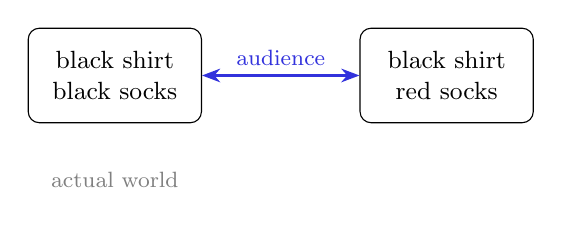
\begin{tikzpicture}[
    world/.style={draw, rounded corners, minimum width=2.2cm, minimum height=1.2cm, align=center, font=\small},
    >=Stealth
  ]
  \node[world, fill=white] (w1) {black shirt\\black socks};
  \node[world, fill=white, right=2cm of w1] (w2) {black shirt\\red socks};
  \draw[thick, agent1, <->] (w1) -- node[above, font=\footnotesize, text=agent1] {audience} (w2);
  \node[below=0.5cm of w1, font=\footnotesize, text=gray] {actual world};
\end{tikzpicture}
\end{center}
\vspace{0.5em}
{\footnotesize
\textcolor{agent0}{I}: no edge $\Rightarrow$ I can tell them apart\\
\textcolor{agent1}{Audience}: edge $\Rightarrow$ can't tell them apart
}
\end{column}
\end{columns}
\end{frame}

% ============================================================
% 2. HOW I GOT HERE (3 min)
% ============================================================

\begin{frame}{How I Got Here}
\begin{itemize}
\item 2025: read Halpern \& Moses, ``Knowledge and Common Knowledge in a Distributed Environment'' (1990, Dijkstra Prize 2009)
\item Started blogging about epistemic logic \& distributed systems
\item Remy Wang organized a seminar here at UCLA on\\Fagin, Halpern, Moses \& Vardi, \emph{Reasoning About Knowledge} (1995)
\item I'm zooming into that seminar --- we're partway through the book
\end{itemize}

\vspace{1em}
\textbf{Joseph Halpern died on February 13, 2026.}\\
His work is foundational to everything in this talk.
\end{frame}

% ============================================================
% 3. THE GAP (2 min)
% ============================================================

\begin{frame}{The Gap}
Epistemic logic is well-developed. But practitioners use \textbf{TLA+}
(Temporal Logic of Actions, Lamport).

\vspace{0.5em}
When we \emph{talk} about distributed algorithms, we say:
\begin{itemize}
\item ``The Raft leader \emph{knows} the entry is replicated''
\item ``The client \emph{doesn't know} if it's safe to retry''
\end{itemize}

\vspace{0.5em}
When we \emph{specify} the algorithm in TLA+, these knowledge statements disappear ---
we write mindless state machines.

\vspace{1em}
\textbf{Can we bridge this gap?}
\end{frame}

% ============================================================
% 4. OUTLINE (30 sec)
% ============================================================

\begin{frame}{Outline}
\begin{enumerate}
\item Epistemic Logic --- $K$, $E$, $C$, $D$ operators
\item TLA+ and TLC --- SimpleRaft as running example
\item My System --- epistemic operators layered on TLA+
\item Comparison with MCMAS
\item Open Questions
\end{enumerate}
\end{frame}

% ============================================================
% 5. EPISTEMIC LOGIC (8 min)
% ============================================================

\begin{frame}{Kripke Structures}
\begin{columns}[T]
\begin{column}{0.5\textwidth}
A Kripke structure is:
\begin{itemize}
\item A set of \textbf{possible worlds} (states)
\item For each agent $i$, an equivalence relation $\sim_i$ (indistinguishability)
\item Agent $i$ \textbf{knows} $\varphi$ iff $\varphi$ holds in all worlds $i$ considers possible
\end{itemize}

\vspace{0.3em}
\textbf{Graph-theoretic view:}\\
Partition the state graph by $\sim_i$.\\
$K_i(\varphi)$ = $\varphi$ holds throughout $i$'s block.
\end{column}
\begin{column}{0.45\textwidth}
\begin{center}
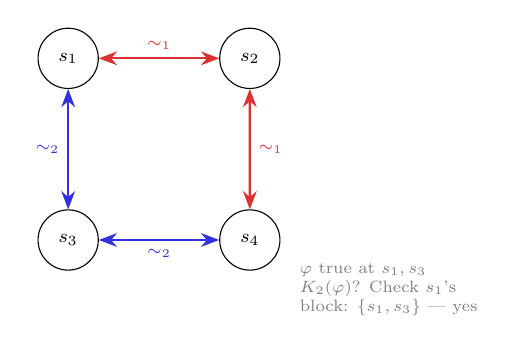
\begin{tikzpicture}[
    world/.style={draw, circle, minimum size=0.9cm, font=\footnotesize, inner sep=1pt},
    >=Stealth,
    scale=0.85, transform shape
  ]
  \node[world] (s1) {$s_1$};
  \node[world, right=1.8cm of s1] (s2) {$s_2$};
  \node[world, below=1.8cm of s1] (s3) {$s_3$};
  \node[world, below=1.8cm of s2] (s4) {$s_4$};

  \draw[thick, agent0, <->] (s1) -- node[above, font=\scriptsize, text=agent0] {$\sim_1$} (s2);
  \draw[thick, agent1, <->] (s3) -- node[below, font=\scriptsize, text=agent1] {$\sim_2$} (s4);
  \draw[thick, agent1, <->] (s1) -- node[left, font=\scriptsize, text=agent1] {$\sim_2$} (s3);
  \draw[thick, agent0, <->] (s2) -- node[right, font=\scriptsize, text=agent0] {$\sim_1$} (s4);

  \node[below right=-0.1cm and 0.3cm of s4, font=\scriptsize, align=left, text=gray] {
    $\varphi$ true at $s_1, s_3$\\
    $K_2(\varphi)$? Check $s_1$'s\\
    block: $\{s_1, s_3\}$ --- yes
  };
\end{tikzpicture}
\end{center}
\end{column}
\end{columns}
\end{frame}

\begin{frame}{Modal Operators}
\begin{description}
\item[$K_i(\varphi)$] Agent $i$ \textbf{knows} $\varphi$\\
{\small $\varphi$ holds at all states in $i$'s equivalence class}
\vspace{0.3em}
\item[$E(\varphi)$] \textbf{Everyone knows} $\varphi$\\
{\small $K_i(\varphi)$ for all agents $i$ \ --- \ intersection of $K$ results}
\vspace{0.3em}
\item[$C(\varphi)$] \textbf{Common knowledge} of $\varphi$\\
{\small Fixed point: $\varphi \wedge E(\varphi) \wedge E(E(\varphi)) \wedge \cdots$\\
Graph reachability on the union of all $\sim_i$}
\vspace{0.3em}
\item[$D(\varphi)$] \textbf{Distributed knowledge} of $\varphi$\\
{\small The group's pooled information --- intersect all agents' equivalence classes}
\end{description}
\end{frame}

\begin{frame}{Nested Knowledge}
\Large
$$K_1(K_2(\varphi))$$

\normalsize
``Agent 1 knows that agent 2 knows $\varphi$''

\vspace{1em}
Evaluated by composition:
\begin{enumerate}
\item Compute where $K_2(\varphi)$ holds (set of states)
\item Compute where $K_1$ of that result holds
\end{enumerate}

\vspace{1em}
\textbf{Key insight:} evaluating knowledge formulas = partitioning the state graph + set operations. No theorem proving needed.
\end{frame}

\begin{frame}{Agent History and Local State}
In the Halpern \& Moses framework:
\begin{itemize}
\item An agent's knowledge is determined by its \textbf{local state} --- everything it has observed
\item \textbf{Perfect recall:} agents remember their entire history
\item Two global states are indistinguishable to agent $i$ iff $i$'s local state is identical in both
\end{itemize}

\vspace{0.8em}
$$s \sim_i s' \iff \text{local\_state}_i(s) = \text{local\_state}_i(s')$$

\vspace{0.8em}
This connects directly to \textbf{graph theory}: no axioms, no theorem proving --- just partition and check.
\end{frame}

% ============================================================
% 6. TLA+ AND TLC (8 min)
% ============================================================

\begin{frame}{TLA+ and TLC}
\textbf{TLA+} = Temporal Logic of Actions (Lamport)
\begin{itemize}
\item A spec defines a state machine: initial states + next-state relation
\item Temporal properties: safety ($\Box\varphi$) and liveness ($\Diamond\varphi$)
\item \textbf{TLC} = model checker --- explores reachable states, checks properties
\item TLC can dump the full state graph to disk (JSON)
\end{itemize}

\vspace{0.5em}
\textbf{PlusCal:} higher-level language that compiles to TLA+
\begin{itemize}
\item Key addition: \textbf{processes} --- named concurrent actors with local variables
\item Processes naturally define \textbf{agents}
\item Process-local variables define what each agent can \textbf{observe}
\end{itemize}
\end{frame}

\begin{frame}[fragile]{SimpleRaft: PlusCal}
{\small A leader replicates a command to two followers, waits for an ack, then commits.}
\begin{lstlisting}[language=tlaplus,basicstyle=\ttfamily\tiny]
process LeaderProc = Leader
variables sent = [f \in Followers |-> FALSE],
          acks = [f \in Followers |-> FALSE],
          commandAcknowledged = FALSE;
begin
    SendFirst:
        with f \in Followers do
            network := network \union {[type |-> "send", dest |-> f]};
            sent[f] := TRUE;
        end with;
    SendSecond:
        with f \in {f \in Followers : ~sent[f]} do
            network := network \union {[type |-> "send", dest |-> f]};
            sent[f] := TRUE;
        end with;
    ReceiveAck1:
        with f \in {f : ack[f] \in network} do acks[f] := TRUE; end with;
    AcknowledgeCommand:
        commandAcknowledged := TRUE;
    ReceiveAck2:
        with f \in {f : ack[f] \in network} do acks[f] := TRUE; end with;
end process;

process FollowerProc \in Followers
variable received = FALSE;
begin
    ReceiveAndAck:
        await [type |-> "send", dest |-> self] \in network;
        received := TRUE;
        network := network \union {[type |-> "ack", src |-> self]};
end process;
\end{lstlisting}
\end{frame}

\begin{frame}{SimpleRaft: Agents and Observable State}
\begin{center}
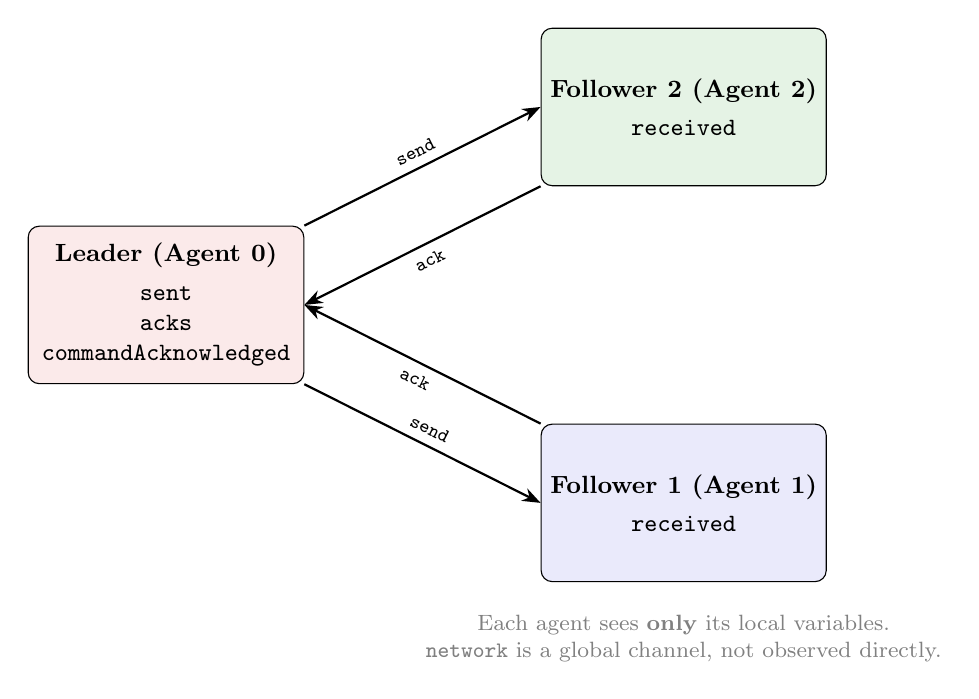
\begin{tikzpicture}[
    box/.style={draw, rounded corners, minimum width=3.5cm, minimum height=2cm, align=center, font=\small},
    msg/.style={->, thick, >=Stealth}
  ]
  \node[box, fill=agent0!10] (leader) {
    \textbf{Leader (Agent 0)}\\[0.3em]
    \texttt{sent}\\
    \texttt{acks}\\
    \texttt{commandAcknowledged}
  };
  \node[box, fill=agent1!10, below right=0.5cm and 3cm of leader] (f1) {
    \textbf{Follower 1 (Agent 1)}\\[0.3em]
    \texttt{received}
  };
  \node[box, fill=agent2!10, above right=0.5cm and 3cm of leader] (f2) {
    \textbf{Follower 2 (Agent 2)}\\[0.3em]
    \texttt{received}
  };
  \draw[msg] (leader.north east) -- node[above, sloped, font=\scriptsize] {\texttt{send}} (f2.west);
  \draw[msg] (f2.south west) -- node[below, sloped, font=\scriptsize] {\texttt{ack}} (leader.east);
  \draw[msg] (leader.south east) -- node[above, sloped, font=\scriptsize] {\texttt{send}} (f1.west);
  \draw[msg] (f1.north west) -- node[below, sloped, font=\scriptsize] {\texttt{ack}} (leader.east);

  \node[below=0.3cm of f1, font=\footnotesize, text=gray, align=center] {
    Each agent sees \textbf{only} its local variables.\\
    \texttt{network} is a global channel, not observed directly.
  };
\end{tikzpicture}
\end{center}
\end{frame}

\begin{frame}{Temporal Properties}
TLC checks temporal properties over state traces:

\vspace{0.3em}
\begin{description}
\item[Safety:] $\Box(\texttt{commandAcknowledged} \Rightarrow \text{majority received})$\\
{\small ``If the command is acknowledged, a majority has received it --- always.''}
\vspace{0.2em}
\item[Liveness:] $\Diamond(\texttt{commandAcknowledged})$\\
{\small ``The command is eventually acknowledged.''}
\vspace{0.2em}
\item[Leads-to:] $\texttt{sent}[1] \leadsto \texttt{received}[1]$\\
{\small ``Once the leader sends to follower 1, follower 1 eventually receives it.''}
\end{description}

\vspace{0.5em}
\textbf{Key observation:} PlusCal processes = agents, local variables = observations.
This is exactly the ``local state'' that epistemic logic needs.
\end{frame}

% ============================================================
% 7. THE KNOWLEDGE GAP IN PRACTICE (3 min)
% ============================================================

\begin{frame}{The Knowledge Gap in Practice}
In everyday speech about Raft:
\begin{itemize}
\item ``The leader \emph{knows} the entry is durable when it gets a majority of acks''
\item ``A follower \emph{knows} about the entry when it receives the message''
\item ``The leader \emph{doesn't know which} follower will ack first''
\end{itemize}

\vspace{0.3em}
In TLA+, none of this is expressed. We write protocol logic about what agents \emph{do}, not what they \emph{know}.

\vspace{0.3em}
Epistemic logic could be particularly useful for:
\begin{itemize}
\item \textbf{Byzantine fault tolerance} --- what can honest nodes know about faulty ones?
\item \textbf{Cryptographic protocols} --- what does an eavesdropper know?
\item \textbf{Security} --- information flow, access control
\end{itemize}
\end{frame}

% ============================================================
% 8. MY SYSTEM (8 min)
% ============================================================

\begin{frame}{System Architecture}
\begin{center}
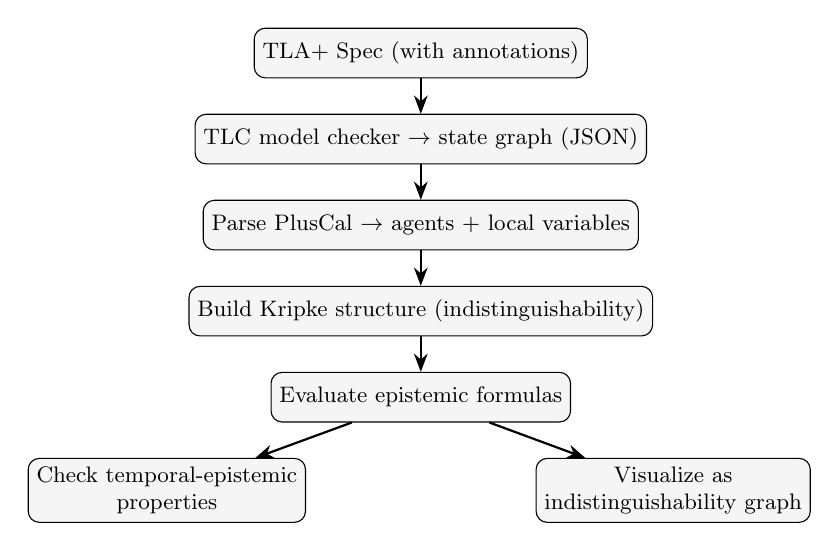
\begin{tikzpicture}[
    box/.style={draw, rounded corners, minimum width=3.5cm, minimum height=0.7cm, align=center, font=\small, fill=codebg},
    arr/.style={->, thick, >=Stealth},
    scale=0.9, transform shape
  ]
  \node[box] (spec) {TLA+ Spec (with annotations)};
  \node[box, below=0.5cm of spec] (tlc) {TLC model checker $\to$ state graph (JSON)};
  \node[box, below=0.5cm of tlc] (parse) {Parse PlusCal $\to$ agents + local variables};
  \node[box, below=0.5cm of parse] (kripke) {Build Kripke structure (indistinguishability)};
  \node[box, below=0.5cm of kripke] (eval) {Evaluate epistemic formulas};
  \node[box, below left=0.5cm and -0.5cm of eval] (check) {Check temporal-epistemic\\properties};
  \node[box, below right=0.5cm and -0.5cm of eval] (viz) {Visualize as\\indistinguishability graph};

  \draw[arr] (spec) -- (tlc);
  \draw[arr] (tlc) -- (parse);
  \draw[arr] (parse) -- (kripke);
  \draw[arr] (kripke) -- (eval);
  \draw[arr] (eval) -- (check);
  \draw[arr] (eval) -- (viz);
\end{tikzpicture}
\end{center}
\end{frame}

\begin{frame}[fragile]{Three Kinds of Annotations}
{\small In TLA+ comments:}

\vspace{0.3em}
\textbf{1. Knowledge Query} --- ``where does this hold?''
\begin{lstlisting}[basicstyle=\ttfamily\tiny]
\* KNOWLEDGE_QUERY K(0, K(1, received[1]) \/ K(2, received[2]))
\end{lstlisting}
\vspace{-0.3em}
{\small Highlights satisfying states on the graph}

\vspace{0.3em}
\textbf{2. Knowledge Property} --- temporal assertion
\begin{lstlisting}[basicstyle=\ttfamily\tiny]
\* KNOWLEDGE_PROPERTY <>K(0, K(1, received[1]) \/ K(2, received[2]))
\end{lstlisting}
\vspace{-0.3em}
{\small PASS/FAIL: combines $\Box$, $\Diamond$, $\leadsto$ with epistemic formulas}

\vspace{0.3em}
\textbf{3. Knowledge Precondition} --- knowledge-based protocol
\begin{lstlisting}[basicstyle=\ttfamily\tiny]
\* KNOWLEDGE_PRECONDITION AcknowledgeCommand: K(0, K(1, received[1]) \/ K(2, received[2]))
\end{lstlisting}
\vspace{-0.3em}
{\small ``The leader only commits when it \emph{knows} a follower knows''}
\end{frame}

\begin{frame}{Demo: SimpleRaft --- Indistinguishability Graph}
\begin{center}
\includegraphics[height=0.85\textheight]{../raft/SimpleRaft-indistinguishability.pdf}
\end{center}
\end{frame}

\begin{frame}[fragile]{Demo: SimpleRaft --- Property Checks}
\begin{lstlisting}[basicstyle=\ttfamily\scriptsize, language={}, backgroundcolor=\color{black!5}]
K(0, (K(1, received[1]) \/ K(2, received[2])))
  holds at 9/18 states

<>K(0, (K(1, received[1]) \/ K(2, received[2]))): PASS
sent[1] ~> K(1, received[1]):                     PASS
sent[2] ~> K(2, received[2]):                     PASS

Precondition AcknowledgeCommand:
  K(0, (K(1, received[1]) \/ K(2, received[2]))):
    PASS (holds at all 4 states)
\end{lstlisting}

\vspace{0.5em}
\begin{itemize}
\item Early states: many indistinguishability edges (leader doesn't know who received what)
\item As acks arrive, edges disappear (leader gains knowledge)
\item At \texttt{AcknowledgeCommand}: leader \emph{knows} a follower knows
\end{itemize}
\end{frame}

\begin{frame}{Demo: Coordinated Attack}
\begin{columns}[T]
\begin{column}{0.42\textwidth}
Two generals, unreliable messenger.

\vspace{0.3em}
Nested knowledge hierarchy:
\begin{itemize}
\item $K_1(\text{rcvd}_1)$ --- 5/7 states
\item $K_0(\text{rcvd}_1)$ --- 4/7 states
\item $K_1(K_0(\text{rcvd}_1))$ --- 3/7
\item $K_0(K_1(K_0(\text{rcvd}_1)))$ --- 2/7
\end{itemize}

\vspace{0.3em}
Each nesting level holds at fewer states.

\vspace{0.3em}
\textbf{But:} $\Box \neg C(\text{rcvd}_1)$ --- PASS\\[0.2em]
Common knowledge is \textbf{never} achieved.

\vspace{0.3em}
{\footnotesize Halpern \& Moses's impossibility result, mechanically verified.}

\end{column}
\begin{column}{0.58\textwidth}
\begin{center}
\includegraphics[width=\textwidth]{../coordinated-attack/CoordinatedAttack-indistinguishability.pdf}
\end{center}
\end{column}
\end{columns}
\end{frame}

\begin{frame}[fragile]{Demo: Coordinated Attack --- The PlusCal}
\begin{lstlisting}[language=tlaplus,basicstyle=\ttfamily\tiny]
process Gen \in Generals
variables sent = 0, rcvd = 0;
begin
    Step:
        while sent < Rounds do
            if self = 0 /\ sent = 0 then
                \* General 0 initiates. Message might be lost.
                with arrives \in {0, 1} do
                    if arrives = 1 then
                        network := network \union {[to |-> 1]};
                    end if;
                end with;
                sent := 1;
            else
                \* Receive, send reply which might be lost.
                await [to |-> self] \in network;
                rcvd := rcvd + 1;
                sent := sent + 1;
                with arrives \in {0, 1} do
                    if arrives = 1 then
                        network := (network \ {[to |-> self]})
                                   \union {[to |-> 1 - self]};
                    else
                        network := network \ {[to |-> self]};
                    end if;
                end with;
            end if;
        end while;
end process;
\end{lstlisting}
\end{frame}

% ============================================================
% 9. COMPARISON WITH MCMAS (3 min)
% ============================================================

\begin{frame}{Comparison with MCMAS}
\textbf{MCMAS} (Lomuscio et al., Imperial College, 2006):
\begin{itemize}
\item Purpose-built epistemic model checker
\item Checks \textbf{CTLK} (branching-time temporal + epistemic operators)
\item Uses \textbf{ISPL} (Interpreted Systems Programming Language)
\item BDD-based symbolic model checking --- doesn't enumerate states
\end{itemize}

\vspace{0.3em}
\textbf{However:}
\begin{itemize}
\item Almost entirely academic --- no industry adoption
\item Development dormant since $\sim$2017
\item TLA+ is the de facto standard for distributed systems
{\small (AWS, Azure, MongoDB, CockroachDB, Confluent, Elastic\ldots)}
\item Nobody is going to rewrite their Raft spec in ISPL
\end{itemize}
\end{frame}

\begin{frame}{My Approach vs.\ MCMAS}
\begin{center}
\renewcommand{\arraystretch}{1.4}
\begin{tabular}{l|l|l}
& \textbf{My approach} & \textbf{MCMAS} \\
\hline
Input & TLA+ / PlusCal & ISPL \\
Community & industry practitioners & academic \\
Algorithm & explicit state graph & BDD-based \\
Scalability & limited (full dump) & better (symbolic) \\
Temporal logic & LTL-like & CTL \\
Status & prototype & dormant \\
\end{tabular}
\end{center}

\vspace{0.5em}
\textbf{Value proposition:} meet practitioners where they are.\\
Layer epistemic analysis on top of specs that \emph{already exist}.
\end{frame}

% ============================================================
% 10. CONCLUSION AND OPEN QUESTIONS (3 min)
% ============================================================

\begin{frame}{What I've Shown}
\begin{itemize}
\item Epistemic logic formalizes the knowledge reasoning we already do informally about distributed algorithms
\item TLA+ specs already contain the structure needed for epistemic analysis\\
(processes = agents, local variables = observations)
\item We can mechanically verify knowledge properties of existing TLA+ specs
\end{itemize}
\end{frame}

\begin{frame}{Open Questions}
\begin{enumerate}
\item \textbf{Is this useful?} Does adding knowledge operators to TLA+ help practitioners design better protocols, or is it just intellectually satisfying?

\vspace{0.3em}
\item \textbf{Scalability:} Epistemic operators need to be evaluated \emph{during} model checking, not as a post-processing step. Is on-the-fly epistemic model checking within TLC a researched problem?

\vspace{0.3em}
\item \textbf{Should we just use MCMAS?} Or is TLA+'s ecosystem worth adding epistemic features to TLC?

\vspace{0.3em}
\item \textbf{What applications would benefit most?}\\
Byzantine fault tolerance? Cryptographic protocols?\\
Information flow security? Mechanism design?
\end{enumerate}
\end{frame}

\begin{frame}{}
\begin{center}
\Huge Thank you

\vspace{1em}
\large Questions?

\vspace{2em}
\normalsize
\url{https://github.com/ajdavis/knowledge-tlaplus}
\end{center}
\end{frame}

% ============================================================
% BACKUP SLIDES
% ============================================================

\appendix

\begin{frame}{References}
\small
\begin{itemize}
\item Halpern \& Moses, ``Knowledge and Common Knowledge in a Distributed Environment'' (JACM 1990)
\item Fagin, Halpern, Moses \& Vardi, \emph{Reasoning About Knowledge} (MIT Press 1995)
\item Lomuscio, Qu \& Raimondi, ``MCMAS: A Model Checker for the Verification of Multi-Agent Systems'' (CAV 2009)
\item van der Meyden et al., ``On the Complexity of Model Checking Knowledge and Time'' (ACM TOCL 2024)
\item Penczek, ``Model Checking Temporal Epistemic Logic'' (2015)
\end{itemize}
\end{frame}

\begin{frame}{Demo: Muddy Children}
\begin{columns}[T]
\begin{column}{0.42\textwidth}
Classic puzzle (Halpern \& Moses~\S2):
\begin{itemize}
\item $N$ children, $k$ muddy
\item Father: ``at least one has mud''
\item Each round: ``do you know?''
\end{itemize}

\vspace{0.3em}
$K(i, \text{muddy}[i])$ first holds at $q = k\!-\!1$:

\vspace{0.2em}
{\small
\begin{tabular}{c|ccc}
& $q\!=\!0$ & $q\!=\!1$ & $q\!=\!2$ \\
\hline
$k\!=\!1$ & K & K & K \\
$k\!=\!2$ & -- & K & K \\
$k\!=\!3$ & -- & -- & K \\
\end{tabular}
}

\vspace{0.3em}
{\small Verified: muddy children know exactly when the algorithm says ``yes''.}
\end{column}
\begin{column}{0.58\textwidth}
\begin{center}
\includegraphics[width=\textwidth]{../muddy-children/MuddyChildren-indistinguishability.pdf}
\end{center}
\end{column}
\end{columns}
\end{frame}

\end{document}
